\documentclass[11pt, a4paper]{article}
\usepackage{tikz}
\usepackage{kotex}
\usepackage{amsthm}
\usepackage{amsmath}
\usepackage{amssymb}
\usepackage{geometry}
\geometry{
    margin=1mm,
    headheight=1mm,
    footskip=10mm
}

\begin{document}
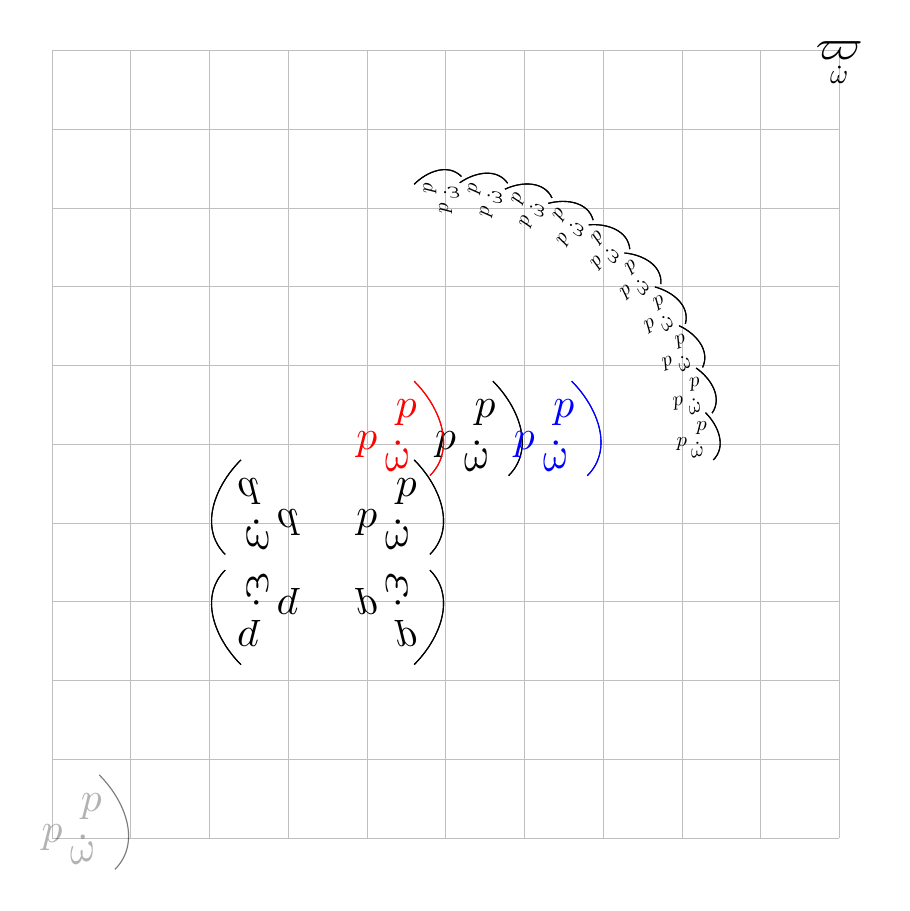
\begin{tikzpicture}[
    cat/.pic={
        \tikzset{every node/.style={transform shape}}%this important feature
        \node[scale=1.5] at (0, 0) {$p$};
        \node[scale=1.5] at (0.5, 0.4) {$p$};
        \node[scale=1.5] at (0.4, 0) {$\cdot$};
        \node[scale=1.5,rotate=15] at (0.4, -0.2) {$\omega$};
        \draw[] (0.6,0.8) to[out=-45, in=45] (0.8,-0.4);
        \draw[] (0.6,0.8) to[out=-45, in=45] (0.8,-0.4);
    }
]
    \draw[help lines, lightgray] (-5,-5) grid (5,5);%guide line

    \pic at (0,0) {cat};
    \pic[blue] at (1,0) {cat};
    \pic[red] at (-1,0) {cat};

    \foreach \x in {0,10,...,90}{
        \pic[rotate=\x,scale=0.5] at (\x:3) {cat};
    }

    \pic at (-1,-1) {cat};
    \pic[xscale=-1] at (-2,-1) {cat};
    \pic[yscale=-1] at (-1,-2) {cat};
    \pic[xscale=-1, yscale=-1] at (-2,-2) {cat};

    \pic[opacity=0.3] at (-5,-5) {cat};

    \begin{scope}[shift={(5,5)}]%direct draw
        \node[xscale=2,yscale=1.5] at (0, 0) {$\varpi $};
        \node[] at (0, -0.23) {$\cdot$};
        \node[rotate=0] at (0, -0.34) {$\omega$};
    \end{scope}
\end{tikzpicture}
\end{document}